\documentclass[10pt,twocolumn]{article}
	
\usepackage{myfontstyle}
\usepackage{mypackages}
\usepackage{mymacros}
\usepackage{mycommands}

\begin{document}
\thispagestyle{fancy1}

%%% Title and Abstract------------------------
\twocolumn[
\begin{center}
	\hrule
	\vspace{3pt}
	% Title:
	{\sffamily\bfseries\Large
		White Paper - A Dynamic Model for AI Adoption and Compute Projection
	} \\
	{\color{gray}
		\vspace{3pt}
		\hrule
		\vspace{3pt}
	}
	{
		\hspace*{\fill}
		Julian Soh and 
		%\hspace*{\fill}
		Priyanshi Singh
		%\hspace*{\fill}
		%Third Author
		\hspace*{\fill}
%		Fourth Author    % uncomment these two lines if there's a fourth author
%		\hspace*{\fill}
	}\\
	\vspace{3pt}
	{\itshape
		\hspace*{\fill}
		Microsoft Corporation
		\hspace*{\fill} \\
		\hspace*{\fill}
		US State, Local, Education (SLED) - Independent Software Vendors
		\hspace*{\fill}
	}\\
	\vspace{3pt}
	{
		\hspace*{\fill}
		\today{} % today's date ... can type manually instead
		\hspace*{\fill}
	}
	\vspace{3pt}
	{\color{gray}\hrule}
%	\vspace{2pt}
\end{center}
% Abstract:
\begin{adjustwidth}{1.5in}{1.5in}
{\small
\noindent\textbf{Abstract.} \hspace{1em}
A dynamic, non-linear model to describe the adoption of any Artificial Intelligence (AI) technology and its corelation to tokens and compute requirements, for the purposes of cost projection and resource allocation.
}
\end{adjustwidth}
\vspace{9pt}
\hrule
\vspace{1\baselineskip}
]

%%% Body -------------------------

\section{Introduction} 
\label{sec:introduction}

The rapid proliferation of AI-powered services—particularly intelligent assistants like Microsoft Copilot—has reshaped digital workflows across industries. Understanding the dynamics of their adoption is critical not only for forecasting market penetration but also for optimizing deployment strategies, licensing models, and infrastructure provisioning (\cite{Soh2024}). Traditional linear models fail to capture the complex, nonlinear nature of user uptake, which is often influenced by network effects, saturation thresholds, external campaigns, and churn.

This paper proposes a mathematical framework to simulate the adoption trajectory of an AI solution. By leveraging a logistic growth model and extending it with token and compute consumption, we aim to provide a data-driven and mathematical approach to making informed decisions regarding resource allocation and pricing strategies.
\section{Methods}

We begin by introducing the canonical logistic growth equation and then progressively extend it to reflect the impact on tokens and/or compute. The resulting approach serves as a reusable template for forecasting, scenario planning, and strategic rollout of AI services in enterprise and consumer contexts.

When extending the analysis to incorporate token consumption, we will take token caching\footnote{Applicable only to newer models such as GPT-4.1 and GPT-5.} into account, thereby leveraging the efficiencies found in newer models. See \autoref{sec:cached-input-tokens} for more details.
\subsection{Logistic Growth Model}
We propose a growth model that reflects user adoption over time. Furthermore, the model needs to capture the fundamental dynamics of user adoption and is expressed as follows:

Let:
\begin{itemize}
\item $A(t)$ be the number of active users at time $t$.
\item $K$ be the carrying capacity, representing the maximum potential user base.
\item $r$ be the intrinsic growth rate, reflecting the natural adoption speed.
\end{itemize}

Then:
\begin{equation}
	\frac{dA}{dt} = r A \left(1 - \frac{A}{K}\right)
	\label{eq:CoreModel}
\end{equation}

\subsection{Assumptions and Limitations}
The following assumptions are made in this model:
\begin{itemize}
	\item We will use a Heuristic model for estimating Cached Input Tokens (for GPT-4.1 and above). See \autoref{sec:cached-input-tokens}.
	\item We will base usage scenarios on multi-agent environments using Agent to Agent (A2A) and/or Model Context Protocol (MCP) as communication protocols because this will:
	\begin{itemize}
		\item more accurately reflect the direction of agentic implementations, and
		\item reflect a more realistic scenario for enterprise implementations of AI services.
	\end{itemize}
	\item Use data from AI adoption, not just LLM based, to model the parameters $K$ and $r$.
	\item We will use Microsoft Azure OpenAI Provisioned Throughput Units (PTU) as representation of compute resources.
\end{itemize}

\subsection{Cached Input Tokens}
\label{sec:cached-input-tokens}
Estimating reuse patterns require observation of historic data from user interaction. However, this data may not be available and/or practical to analyze. As such, we will use a heuristic model to estimate the number of cached input tokens.

The Heuristic model for estimating cached input tokens is as follows:
\begin{itemize}
	\item P = average number of prompt tokens
	\item  C - average number of completion tokens
	\item $T_{\text{cached}}$ = average number of cached input tokens
\end{itemize}
Caching only comes into effect when:
\[P \geq 1024\]
If not, then:
\[T_{\text{cached}} = 0\]

Furthermore, the reuse rate of tokens, known as the reuse ratio, $R$ is dependent on the system's configuration:
\begin{itemize}
	\item Static System prompt + reusued instructions: $R = 0.8$
	\item Semi-dynamic prompts (e.g. templated prompts): $R = 0.5$
	\item Highly dynamic prompts: $R = 0.3$
\end{itemize}

Using the values of $P$, $C$ and $R$, we can estimate the average number of cached input tokens, $T_{\text{cached}}$ as follows:
Caching occurs at 128-token blocks $B$ beyond 1,024 tokens. Thus:

\begin{equation}
T_{\text{cached}} =
\begin{cases}
0, & \text{if } P < T_{\text{min}} \\
B \cdot \left\lfloor \frac{\min(R \cdot P, P)}{B} \right\rfloor, & \text{if } P \geq T_{\text{min}}
\end{cases}
\label{eq:Tcached}
\end{equation}

$T_{\text{cached}}$ only \emph{applies to \textbf{prompt tokens}.}


\subsection{Expected Outcomes}
The expected outcome from this model is a description of a slow start, followed by exponential adoption before reaching equilibrium, as depicted by \autoref{fig:growth-model}.
The factors contributing to this characteristic of equilibrium are:
\begin{itemize}
	\item \textbf{Retraction from initial hype:} As the noveltyof the new service wears off, there may be an over-correction in adoption rates that led to the peak.
	\item \textbf{Recovery:} A recovery due to re-engagement and/or late adopters.
	\item \textbf{Stabilization:} The final plateau representing a stable core of user base.
\end{itemize}

\begin{figure}[bt]
	\centering
	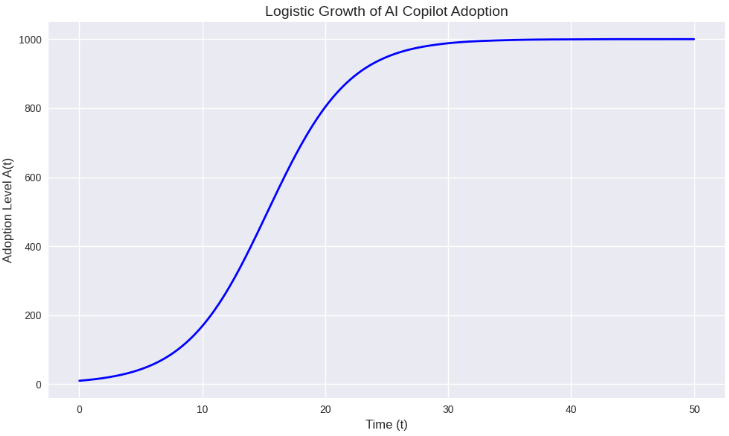
\includegraphics[width=.9\linewidth]{figures/growth-model.png}
	\caption{Ideal AI adoption growth model.}
	\label{fig:growth-model}
\end{figure}

However, in reality, we expect a deviation from this ideal model at the equilibrium (maximum adoption) phase, which,
starting near saturation, dipping due to early churn or fatigue, then rising again and stabilizing\footnote{For this paper, the topic of interest is the adoption rate, so we will exclude the oscillary behavior towards equilibrium.}. It mimics a damped sinusoidal pattern,
as depicted by \autoref{fig:adoption-oscillary-equilibrium}.

\begin{figure}[bt]
	\centering
	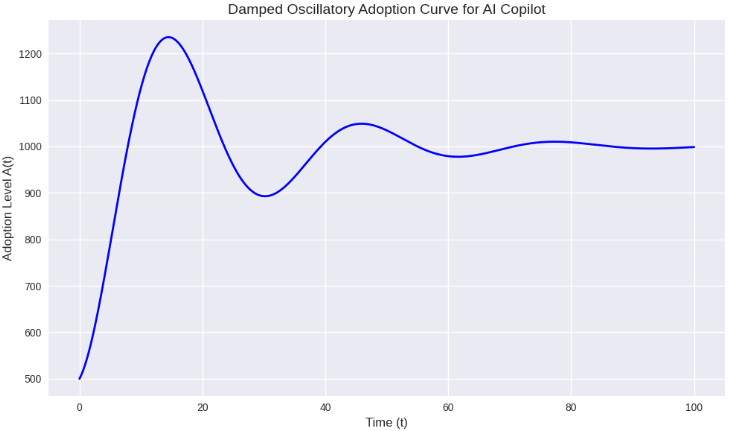
\includegraphics[width=.9\linewidth]{figures/Adoption-oscillary-equilibrium.png}
	\caption{Expected growth model.}
	\label{fig:adoption-oscillary-equilibrium}
\end{figure}

\section{Discussion}
In this section, we will apply our model to a hypothetical AI adoption scenario, demonstrating its utility in forecasting user growth and compute/token requirements.
\subsection{Scenario Definition}
Consider a new AI product aimed at software developers, with a total target of 350,000 users. We will use our model to project user growth over the first year, taking into account the factors identified in our analysis.

As mentioned in our assumptions, we will benchmark our model using multi-agent environments with A2A and/or MCP communication protocols. 
The observed token usage per interaction in a multi-agent, multi-protocol scenario is shown in \autoref{tab:Multi-Agentic}.
\begin{table}[ht]
\scriptsize   % Reduce text size for fitting in one column
\setlength{\tabcolsep}{4pt} % Reduce column padding
\renewcommand{\arraystretch}{1.1} % Slightly tighter row spacing
\centering
\begin{tabularx}{\columnwidth}{ l X c c c }
\hline
\textbf{Source} & \textbf{Scenario} & \textbf{Prompt} & \textbf{Completion} & \textbf{Total} \\
\hline
AgentTaxo\\(\cite{wang2025agenttaxo}) 
& Planner, Reasoner, Verifier roles 
& 8k--15k & 1k--2k & 10k--17k \\

MultiAgentBench\\(\cite{zhu2025multiagentbenchevaluatingcollaborationcompetition})
& Coordination topologies (star, chain, tree, graph) 
& 5k--12k & 800--2k & 6k--14k \\

Reliable Decision-Making\\(\cite{Xian2025})
& Redundant agent deployments (voting, decentralized) 
& 10k--18k & 1k--3k & 12k--21k \\

MCP-Enabled Agents\\(\cite{ding2025networksystemsperformancecharacterization})
& Multi-agent orchestration via Model Context Protocol 
& 8k--20k & 1k--3k & 10k--25k \\
\hline
\end{tabularx}
\caption{Observed Token Utilization in Multi-Agent LLM Systems}
\label{tab:Multi-Agentic}
\end{table}

\subsection{Model Application}
\begin{enumerate}
	\item Parameterization of the logistic growth model
	\item Express users as a function of time
	\item Compute token consumption metrics
	\item Map tokens to token-based and compute-based (PTU) models
\end{enumerate}

\subsubsection{Parameterization of the Logistic Growth Model}

To simulate AI adoption dynamics, we base our model on publicly available data from the February 2025 Federal Reserve's FEDS Notes\footnote{{https://www.federalreserve.gov/econres/notes/feds-notes/measuring-ai-uptake-in-the-workplace-20240205.html}} (\cite{FEDSNotes2025}). This report aggregates 16 surveys conducted between late 2023 and mid-2024, offering a comprehensive view of generative AI uptake across U.S. firms and workers. Firm-level adoption rates vary widely, with the U.S. Census Bureau's BTOS survey reporting less than 5\% of firms using AI in the prior two weeks, while other sources suggest adoption levels as high as 40\%.

For modeling purposes, we define the carrying capacity \( K \) as the maximum potential user base. In our primary simulation, we set \( K = 350{,}000 \) to reflect a large-scale deployment scenario. The initial adoption level \( A_0 \) is set at 5\% of \( K \), yielding \( A_0 = 17{,}500 \) users. This conservative estimate is grounded in the lower bound of observed adoption from the BTOS survey and ensures the model captures the steep acceleration phase typical of early-stage technology uptake. The adoption level after six months is taken as 40\% of \( K \), consistent with upper-bound estimates from aggregated survey data, giving \( A[6] = 140{,}000 \) users.

To estimate the intrinsic growth rate \( r \), we derive the closed-form solution of \autoref{eq:CoreModel}:

\begin{equation}
	A(t) = \frac{K}{1 + \left( \frac{K - A_0}{A_0} \right) e^{-rt}}
\label{eq:ClosedForm}
\end{equation}
\textbf{Given:}
\begin{align*}
A_0 &= 17{,}500 \quad \text{(initial adoption)} \\
A(6) &= 140{,}000 \quad \text{(adoption after 6 months)} \\
K &= 350{,}000 \quad \text{(carrying capacity)}
\end{align*}

Solving numerically for \( r \) using \autoref{eq:ClosedForm}, we obtain:


\[
r \approx 0.4232 \text{ per month}
\]	



For comparison, if we instead use the BTOS sample size as the carrying capacity—approximately 1.2 million firms\footnote{While the U.S. Census Bureau's BTOS survey defines the total population \( K \) as the number of employer firms (approximately 1{,}200{,}000), our model uses \( K = 350{,}000 \) to represent the number of individual users or seats within a specific deployment context. Although these definitions differ---firm-level versus user-level---the logistic growth structure remains valid, as the model is scale-invariant under consistent adoption ratios. This distinction does not materially affect the shape or interpretability of the adoption curve, provided that \( A_0 \) and \( A(t) \) are defined proportionally within the chosen reference frame.}
—the same adoption trajectory yields a slightly higher growth rate of \( r \approx 0.446 \). While both values are close, we adopt the lower \( r \) value in our model to reflect a more conservative adoption rate. This choice allows for cautious forecasting and avoids overestimating infrastructure demand in early rollout phases.

This model provides a reusable framework for forecasting AI service demand, correlating user growth by month modeled using the BTOS survey data, as shown in \autoref{fig:BTOS-350k}.
\begin{figure}[bt]
	\centering
	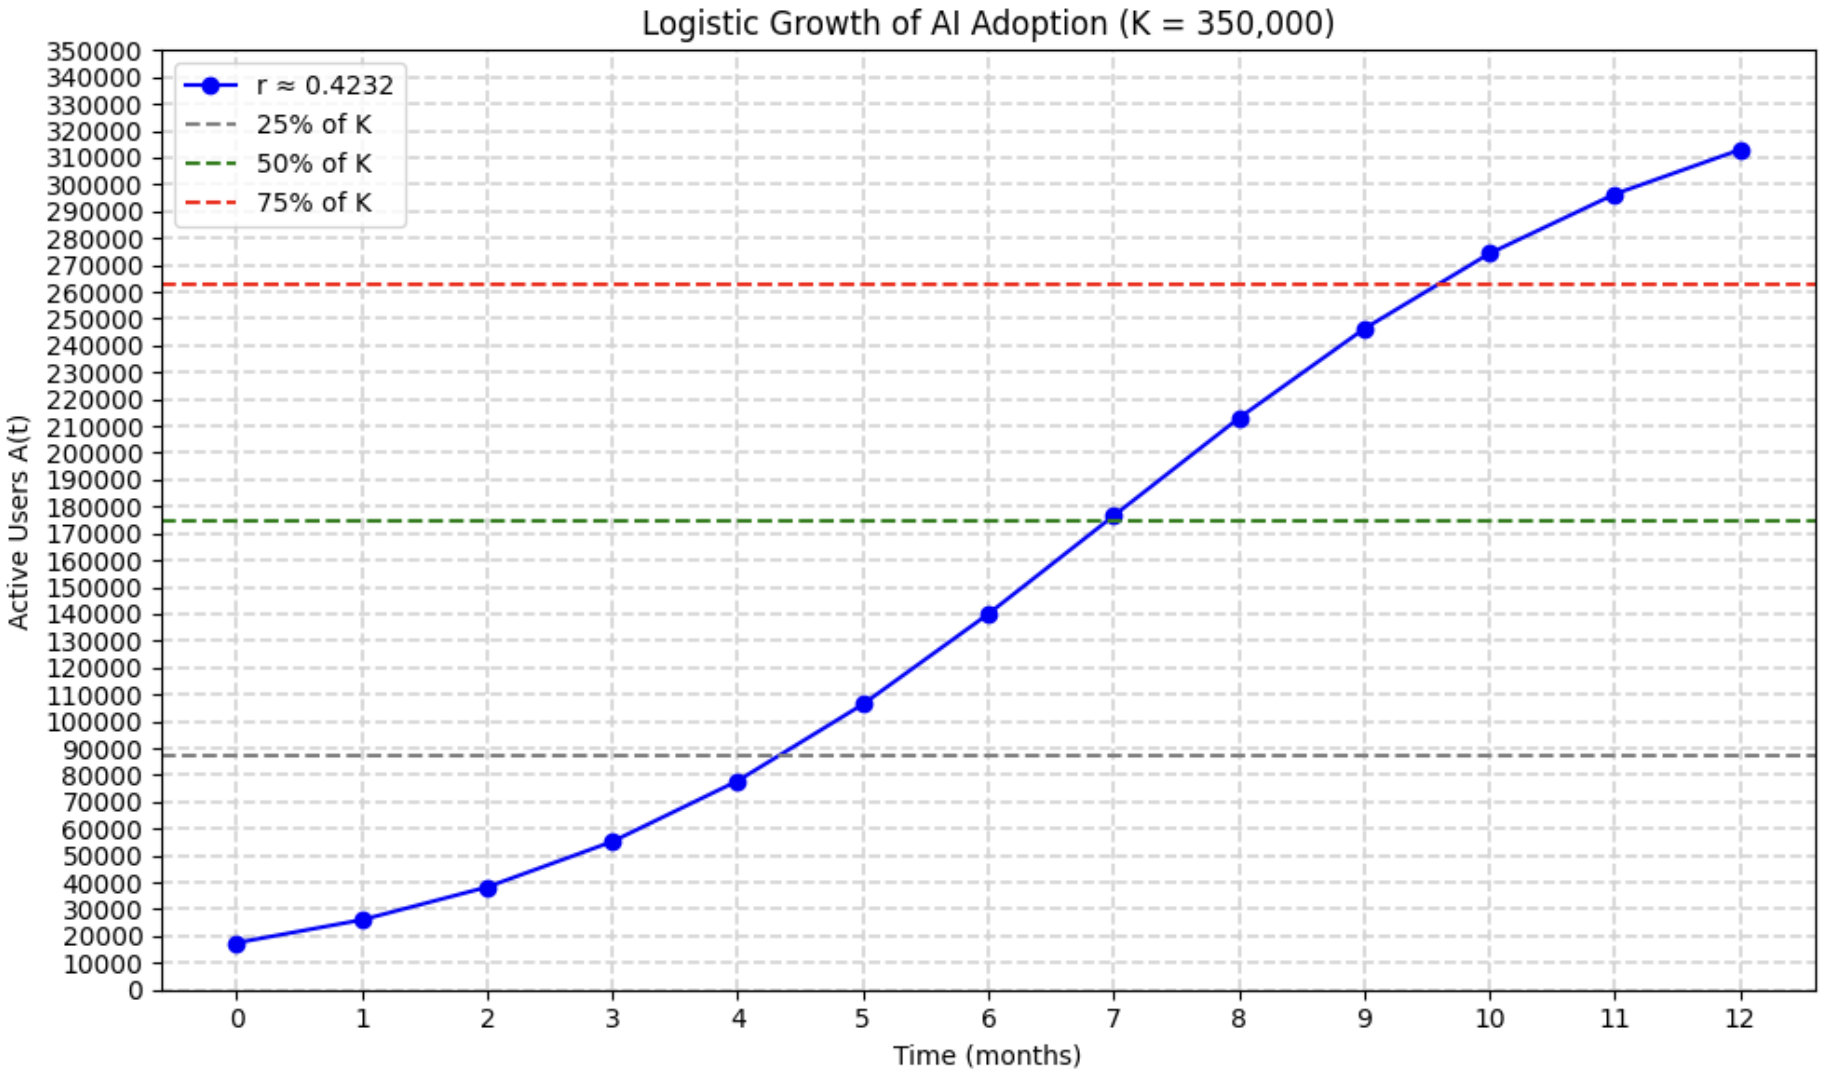
\includegraphics[width=.9\linewidth]{figures/BTOS-Model-350k.png}
	\caption{Adoption Rate for k=350,000.}
	\label{fig:BTOS-350k}
\end{figure}

\subsubsection{Express Users as a Function of Time}
\begin{table}[h!]
\centering
\begin{tabular}{@{}ccc@{}}
\toprule
\textbf{Month} & \textbf{Number of users $A(t)$} \\
\midrule
0  & 17{,}500 \\
1  & 26{,}033 \\
2  & 38{,}248 \\
3  & 55{,}218 \\
4  & 77{,}837 \\
5  & 106{,}377 \\
6  & 140{,}000 \\
7  & 176{,}548 \\
8  & 212{,}962 \\
9  & 246{,}225 \\
10 & 274{,}285 \\
11 & 296{,}408 \\
12 & 312{,}941 \\
\bottomrule
\end{tabular}
\caption{Monthly User Adoption Estimates (K = 350{,}000, $r \approx 0.4232$)}
\label{tab:adoption-daily}
\end{table}

\bigskip

Table~\ref{tab:adoption-daily} presents the monthly adoption levels derived from the closed-form logistic growth model with $K = 350{,}000$ and $r \approx 0.4232$. 
This shows, for example, that on initial launch targeting 350,000 users, we should expect that potentially up to 17,500 users will access the service at any time.

However, in reality, not all 17,500 users will access the service at the same time, so 17,500 Transactions per minute (TPM) is an unlikely scenario. 
We can take a percentage of these users as actual users that will access the service per day, but for the sake of discussion, we will assume that 17,500 users
will access the service per day.

\subsubsection{Compute Token Consumption Metrics}
If we use the token estimates from  \autoref{tab:Multi-Agentic} and average the prompt tokens for our multi-agentic AI-enabled service 
to be 10,000 tokens, and completion tokens to be 2,000 tokens. Now let us also assume we will be using the newer models that have token caching 
capabilities and that we are using a semi-dynamic prompt, so $R = 0.5$. Let us also assume that the 17,500 users will access the service across an 8-hour workday and there are
21 workdays in a month.

Therefore:

\begin{align*}
Users/hour &= \frac{17,500}{8} = 2187.5 \quad \\
Users/minute &= \frac{2187.5}{60} \approx 36 \quad \\
R &= 0.5 \quad \\
T_{prompt}/minute &= (36 \times 10,000 )\cdot0.5 = 180,000 \quad \\
T_{cached}/minute &=  (36 \times 10,000)\cdot0.5 = 180,000 \quad \\
T_{completion}/minute &= 36 \times 2,000 = 72,000 \\
\end{align*}

\begin{figure}[bt]
	\centering
	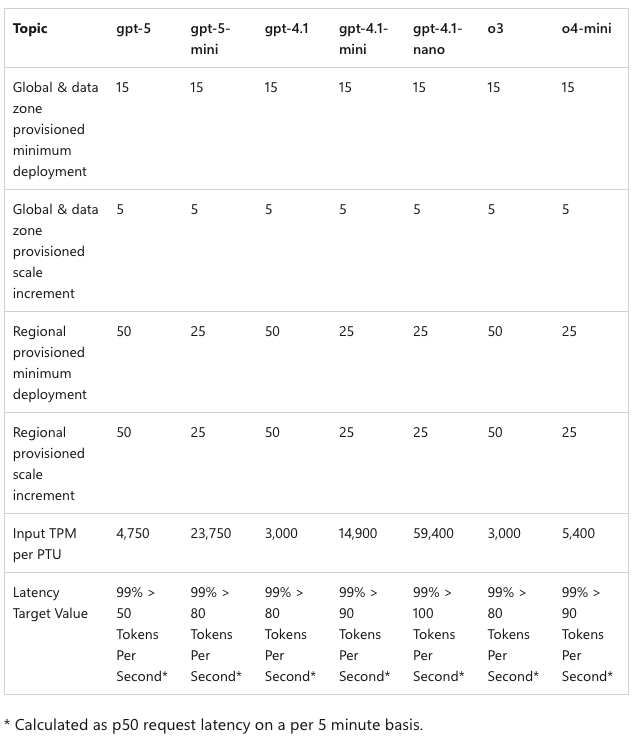
\includegraphics[width=.9\linewidth]{figures/PTU-details-table.png}
	\caption{Latest Azure OpenAI models - PTU details.}
	\label{fig:PTU-details-table}
\end{figure}

Using \emph{Input TPM per PTU}\footnote{Source of table and PTU details for other models located at \url{https://learn.microsoft.com/en-us/azure/ai-services/cognitive-services-usage-pricing/pricing-models/openai-pricing-models}}
from \autoref{fig:PTU-details-table}, we can now estimate the compute requirements for our AI-enabled service.

\begin{table}[ht]
\scriptsize
\setlength{\tabcolsep}{4pt}
\renewcommand{\arraystretch}{1.1}
\centering
\begin{tabularx}{\columnwidth}{ l c c c}
\hline
\textbf{Model} & \textbf{Min PTUs (Global+DZ/Regional)} & \textbf{TPM/PTU} & \textbf{PTUs needed} \\
\hline
gpt-5   & 15/50 & 4{,}750 & 38 \\
gpt-4.1 & 15/50 & 3{,}000 & 60 \\
\hline
\end{tabularx}
\caption{TPM per PTU by Model}
\label{tab:TPM-5-and-4.1}
\end{table}

\autoref{tab:TPM-5-and-4.1} shows our calculations for the number of PTUs needed based on $T_{prompt}/minute = 180,000$ factoring savings from $T_{cached}/minute$.
For gpt-5, we will need at least 38 PTUs to handle the prompt tokens, and for gpt-4.1, we will need at least 60 PTUs because of the latter model's smaller context window.
Furthermore, PTUs have a minimum initial alloocation requirement. Each model also has minimum increment requirements. For Global and Data Zone deployments of gpt-5 and gpt-4.1,
the initial minimum allocation requirement for both models is 15 PTUs with increments of 5 PTUs. 
For Regional deployments, both gpt-5 and gpt-4.1 have an initial minimum allocation requirement of 50 PTUs with increments of 50 PTUs.

Therefore, it is not possible to allocate 38 PTUs of gpt-5 and we will need to round it up to 40 PTUs, in which case
we can allocate 30 Data Zone PTUs with 10 increment PTUs. For gpt-4.1, we can allocate 60 Data Zone PTUs.

If a regional requirement is desired, then gpt-5 will need to be at 50 PTUs. For gpt-4.1, we will need to provision 50 PTUs
and handle excess load with PayGo or to 15 Data Zone PTUs.

These are examples of how you can allocate PTUs based on the adoption model and token consumption estimates.

\section{Conclusion}
In this paper, we presented a non-linear model for AI adoption based on a logistic growth framework based on observed data from the FEDS Notes AI adoption survey.
The model is dynamic by changing the parameters $K$ and $r$ based on different deployment scenarios. The model also
incorporates token consumption based on multi-agentic scenarios and factoring in token caching found in newer models.

%%% References -------------------------
\bibliographystyle{plainnat}
\bibliography{report}

%%% Appendices -------------------------

\end{document}  